\documentclass{article}%
\usepackage[T1]{fontenc}%
\usepackage[utf8]{inputenc}%
\usepackage{lmodern}%
\usepackage{textcomp}%
\usepackage{lastpage}%
\usepackage{geometry}%
\geometry{margin=0.2in}%
\usepackage{graphicx}%
%
\title{Report on Customers dataset}%
\author{Classify2TeX}%
\usepackage{amsmath}%
\usepackage{amssymb}%
\usepackage{enumitem}%
%
\begin{document}%
\normalsize%
\maketitle%
\newpage%
\tableofcontents%
\newpage%
\section{Exploratory Data Analysis}%
\label{sec:ExploratoryDataAnalysis}%
\subsection{Non{-}Null Count, Dtype of features}%
\label{subsec:Non{-}NullCount,Dtypeoffeatures}%
The table 1 provides information about the dataset, including the number of non-null values and the data types of each feature.%


\begin{table}[h!]%
\caption{Dataset Columns Information}%
\vspace{0.2cm}%
\centering%
\begin{tabular}{|c||c||c||c|}%
\hline%
Index&Column&Non{-}Null Count&Dtype\\%
\hline%
0&Customer\_ID&4000&object\\%
1&Age&4000&int64\\%
2&Gender&4000&object\\%
3&Annual\_Income&4000&int64\\%
4&Spending\_Score&4000&int64\\%
5&Region&4000&object\\%
6&Marital\_Status&4000&object\\%
7&Num\_of\_Children&4000&int64\\%
8&Employment\_Status&4000&object\\%
9&Credit\_Score&4000&int64\\%
10&Online\_Shopping\_Frequency&4000&int64\\%
11&Target&4000&int64\\%
\hline%
\end{tabular}%
\end{table}

%
\newpage%
\subsection{Descriptive Statistics}%
\label{subsec:DescriptiveStatistics}%
The table 2 provides descriptive statistics for the dataset, including the count, mean, standard deviation, minimum, and maximum values.%


\begin{table}[h!]%
\caption{Dataset Descriptive Statistics}%
\vspace{0.2cm}%
\centering%
\begin{tabular}{|c||c||c||c||c||c||c||c||c||c|}%
\hline%
Index&Column Name/Statistic&count&mean&std&min&25\%&50\%&75\%&max\\%
\hline%
0&Age&4000.0&43.63&14.96&18.0&31.0&43.0&57.0&69.0\\%
1&Annual\_Income&4000.0&85708.03&37977.69&20076.0&53163.75&85592.5&119030.0&149989.0\\%
2&Spending\_Score&4000.0&49.78&29.01&1.0&25.0&49.0&75.0&99.0\\%
3&Num\_of\_Children&4000.0&1.97&1.4&0.0&1.0&2.0&3.0&4.0\\%
4&Credit\_Score&4000.0&575.12&158.68&300.0&438.0&574.0&712.0&849.0\\%
5&Online\_Shopping\_Frequency&4000.0&9.6&5.78&0.0&5.0&10.0&15.0&19.0\\%
6&Target&4000.0&0.3&0.46&0.0&0.0&0.0&1.0&1.0\\%
\hline%
\end{tabular}%
\end{table}

%
\newpage%
\subsection{Distribution of features}%
\label{subsec:Distributionoffeatures}%
This section provides a visual representation of the distribution of features in the dataset using histograms (numerical features) and bar charts (categorical features). These visualizations can help in understanding the data.%
\subsubsection{Histograms of Numerical columns}%
\label{ssubsec:HistogramsofNumericalcolumns}%
The histograms below show the distribution of numerical features in the dataset.%


\begin{figure}[h!]%
\centering%
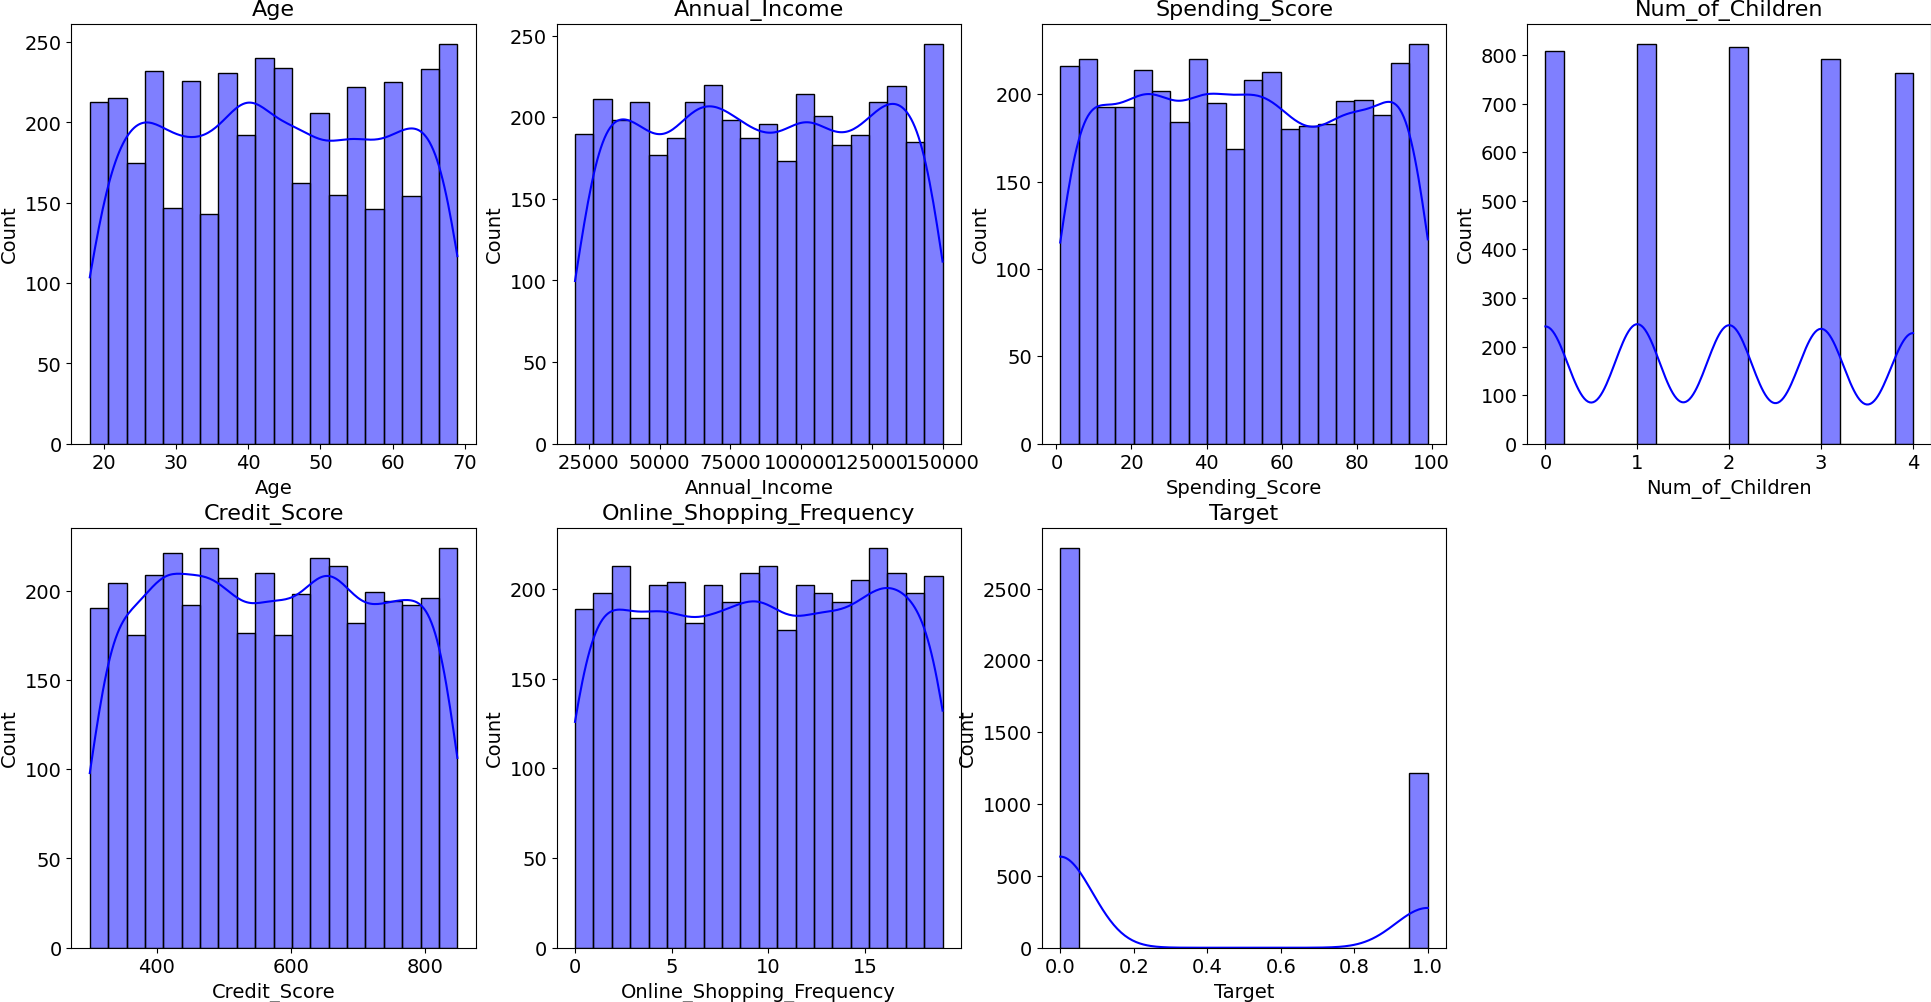
\includegraphics[width=460px]{EDA/histograms.png}%
\caption{Histograms of Numerical columns}%
\end{figure}

%
\newpage%
\subsubsection{Bar Charts of Categorical columns}%
\label{ssubsec:BarChartsofCategoricalcolumns}%
The bar charts below show the distribution of categorical features in the dataset.%


\begin{figure}[h!]%
\centering%
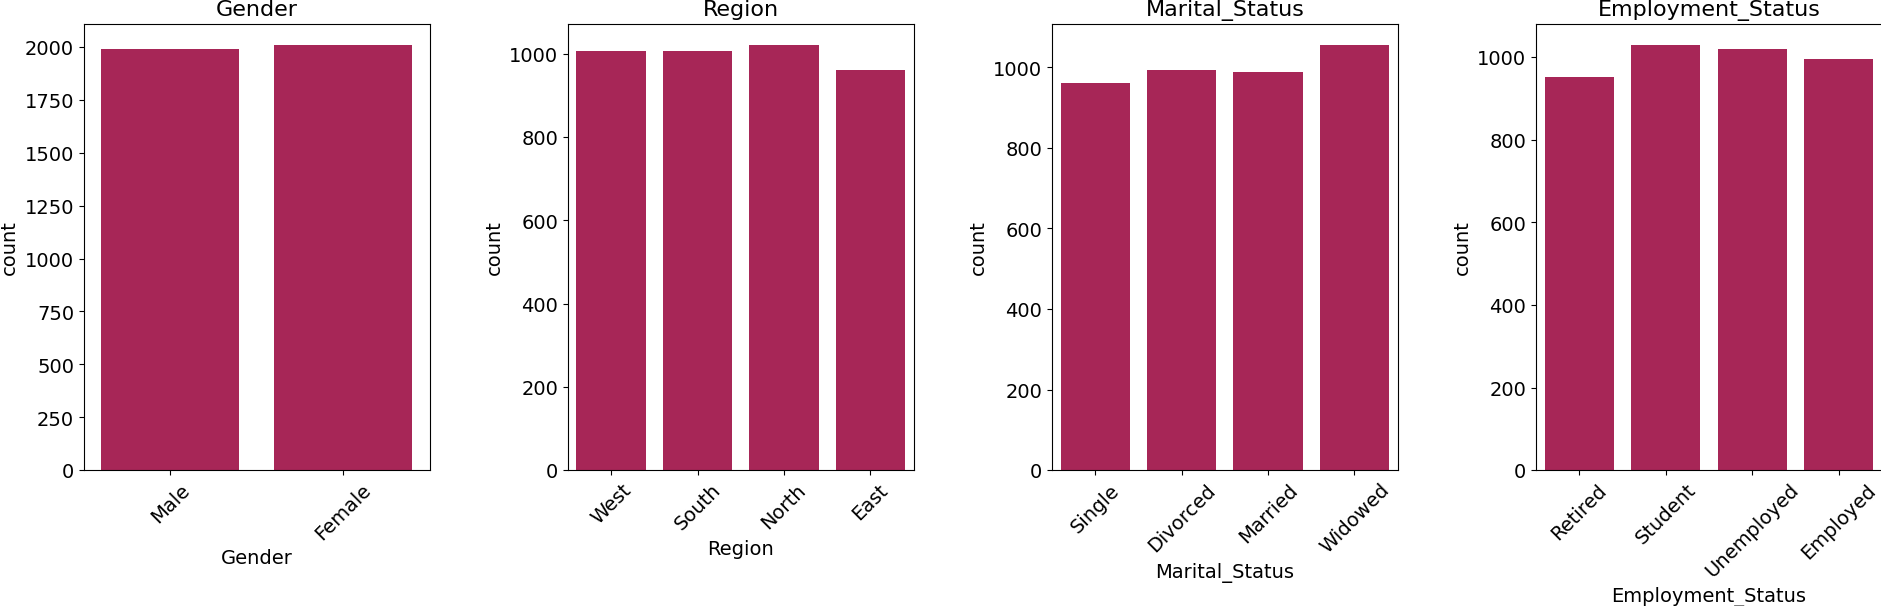
\includegraphics[width=460px]{EDA/bar_charts.png}%
\caption{Bar Charts of Categorical columns}%
\end{figure}

%
\newpage%
\section{Evaluation Metrics}%
\label{sec:EvaluationMetrics}%
\subsection{Accuracy}%
\label{subsec:Accuracy}%

                \textbf{Accuracy} is one of the simplest evaluation metrics for classification models. 
                It is defined as the ratio of correctly predicted observations to the total number of observations:

                \[
                \text{Accuracy} = \frac{\text{Number of Correct Predictions}}{\text{Total Number of Predictions}}
                \]

                While accuracy is intuitive and easy to understand, it may not be suitable for imbalanced datasets. 
                For example, in a dataset where 95\% of the samples belong to one class, predicting the majority class for every instance 
                would result in high accuracy but poor performance on the minority class.
                

%
\subsection{F1 Score}%
\label{subsec:F1Score}%

                The \textbf{F1 Score} is the harmonic mean of Precision and Recall, providing a balance between the two. 
                It is particularly useful when dealing with imbalanced datasets. Precision and Recall are defined as follows:

                \[
                \text{Precision} = \frac{\text{True Positives}}{\text{True Positives} + \text{False Positives}}
                \]
                \[
                \text{Recall} = \frac{\text{True Positives}}{\text{True Positives} + \text{False Negatives}}
                \]

                The F1 Score combines these metrics:

                \[
                \text{F1 Score} = 2 \cdot \frac{\text{Precision} \cdot \text{Recall}}{\text{Precision} + \text{Recall}}
                \]

                A high F1 Score indicates a good balance between Precision and Recall, making it a valuable metric in scenarios where false positives 
                and false negatives have significant costs.
                

%
\subsection{ROC AUC}%
\label{subsec:ROCAUC}%

                The Receiver Operating Characteristic (ROC) curve plots the True Positive Rate (Recall) against the False Positive Rate at various threshold settings. 
                The \textbf{Area Under the Curve (AUC) of the ROC curve} measures the overall ability of the model to distinguish between classes. 

                \[
                \text{AUC} = \int_{\text{FPR}=0}^{1} \text{TPR}(\text{FPR}) \, d(\text{FPR})
                \]

                Key points about ROC AUC:
                \begin{itemize}
                    \item An AUC of 0.5 indicates random guessing.
                    \item An AUC of 1.0 indicates perfect classification.
                    \item It is a threshold-independent metric, providing an aggregate measure of performance across all classification thresholds.
                \end{itemize}

                ROC AUC is particularly useful for binary classification tasks and provides insights into the trade-off between sensitivity and specificity.
                

%
\newpage%
\section{Model Optimization Results}%
\label{sec:ModelOptimizationResults}%
\subsection{Optimization Results Tables}%
\label{subsec:OptimizationResultsTables}%


\begin{table}[h!]%
\caption{Random Forest Hyperparameters and achivied metrics}%
\vspace{0.2cm}%
\centering%
\begin{tabular}{|c||c||c||c||c||c||c||c||c||c|}%
\hline%
Index&Metric/Hyperp.\textbackslash{} Iteration&0&1&2&3&4&5&6&7\\%
\hline%
0&f1&0.886&0.5615&0.861&0.6505&0.8398&0.8543&0.5622&0.5908\\%
1&accuracy&0.886&0.5618&0.861&0.6505&0.8398&0.8543&0.5625&0.5912\\%
2&roc\_auc&0.9286&0.5873&0.9164&0.7124&0.9054&0.9097&0.5822&0.6448\\%
3&n\_estimators&100&200&50&50&50&200&50&500\\%
4&criterion&gini&entropy&entropy&gini&log\_loss&entropy&entropy&entropy\\%
5&max\_depth&None&30&None&20&30&20&20&10\\%
6&min\_samples\_split&2&5&2&10&2&10&5&5\\%
7&min\_samples\_leaf&1&1&2&1&4&2&4&1\\%
8&min\_weight\_fraction\_leaf&0.0&0.05&0.0&0.01&0.0&0.0&0.05&0.0\\%
9&max\_features&sqrt&sqrt&sqrt&log2&None&sqrt&log2&None\\%
10&bootstrap&1&1&1&0&1&1&1&0\\%
\hline%
\end{tabular}%
\end{table}

%


\begin{table}[h!]%
\caption{Decision Tree Hyperparameters and achivied metrics}%
\vspace{0.2cm}%
\centering%
\begin{tabular}{|c||c||c||c||c||c||c||c||c||c|}%
\hline%
Index&Metric/Hyperp. \textbackslash{} Iteration&0&1&2&3&4&5&6&7\\%
\hline%
0&f1&0.7972&0.7188&0.7351&0.4834&0.4834&0.4834&0.6168&0.4834\\%
1&accuracy&0.7998&0.7204&0.7378&0.4885&0.4885&0.4885&0.6182&0.4885\\%
2&roc\_auc&0.7998&0.764&0.7711&0.4857&0.4857&0.4857&0.664&0.4857\\%
3&criterion&gini&entropy&gini&log\_loss&gini&entropy&entropy&entropy\\%
4&splitter&best&random&random&best&random&random&random&random\\%
5&max\_depth&None&30&None&10&10&20&40&10\\%
6&min\_samples\_split&2&5&2&5&10&2&10&5\\%
7&min\_samples\_leaf&1&1&2&4&1&2&4&1\\%
8&max\_features&None&sqrt&None&None&None&None&log2&log2\\%
9&class\_weight&None&balanced&balanced&None&None&None&balanced&None\\%
10&min\_impurity\_decrease&0.0&0.0&0.0&0.01&0.05&0.05&0.0&0.1\\%
\hline%
\end{tabular}%
\end{table}

%


\begin{table}[h!]%
\caption{XGBoost Hyperparameters and achivied metrics}%
\vspace{0.2cm}%
\centering%
\begin{tabular}{|c||c||c||c||c||c||c||c||c||c|}%
\hline%
Index&Metric/Hyperp. \textbackslash{} Iteration&0&1&2&3&4&5&6&7\\%
\hline%
0&f1&0.8186&0.8148&0.7771&0.7071&0.6275&0.8354&0.8173&0.8376\\%
1&accuracy&0.8196&0.8156&0.7771&0.7078&0.6277&0.8357&0.8179&0.8378\\%
2&roc\_auc&0.8949&0.8953&0.8563&0.7666&0.6762&0.91&0.8863&0.91\\%
3&eval\_metric&logloss&logloss&logloss&logloss&logloss&logloss&logloss&logloss\\%
4&n\_estimators&100&500&50&500&200&500&100&200\\%
5&max\_depth&6&15&10&3&3&10&15&10\\%
6&learning\_rate&0.3&0.1&0.01&0.2&0.2&0.05&0.2&0.1\\%
7&subsample&1.0&0.5&0.9&0.7&0.5&0.9&1.0&0.7\\%
8&colsample\_bytree&1.0&0.9&0.5&0.5&0.5&0.7&0.7&0.7\\%
9&min\_child\_weight&1&5&1&1&5&1&7&1\\%
10&gamma&0.0&0.0&0.1&0.1&0.2&0.1&0.0&0.2\\%
11&reg\_alpha&0.0&0.0&0.1&0.1&1.0&1.0&1.0&0.0\\%
12&reg\_lambda&1.0&5.0&1.5&2.0&2.0&5.0&1.0&5.0\\%
\hline%
\end{tabular}%
\end{table}

%
\newpage%
\subsection{Boxplots of accuracy, f1, roc\_auc}%
\label{subsec:Boxplotsofaccuracy,f1,rocauc}%


\begin{figure}[h!]%
\centering%
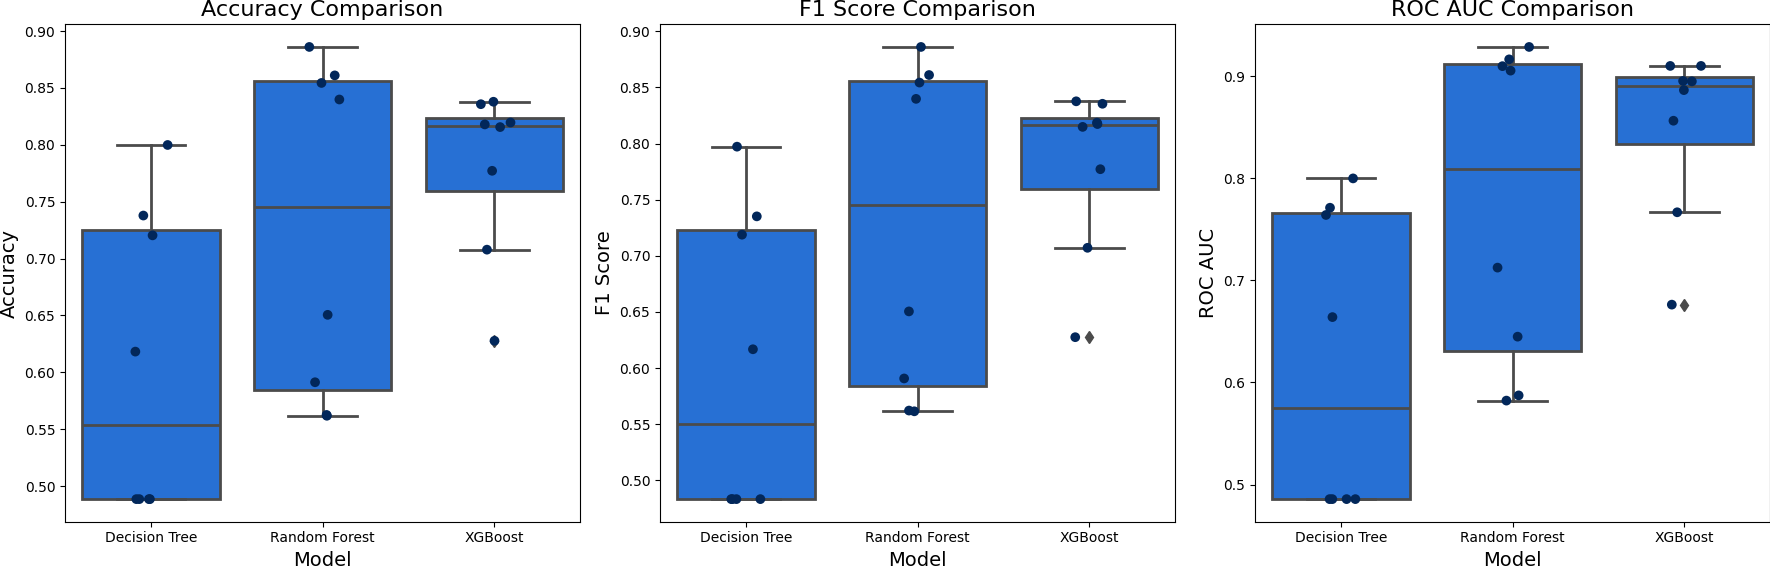
\includegraphics[width=460px]{ModelOptimization/box_plots_metrics.png}%
\caption{Boxplots of accuracy, f1, roc\_auc}%
\end{figure}

%
\subsection{Barplots of maximum values of metrics achievied by model}%
\label{subsec:Barplotsofmaximumvaluesofmetricsachieviedbymodel}%


\begin{figure}[h!]%
\centering%
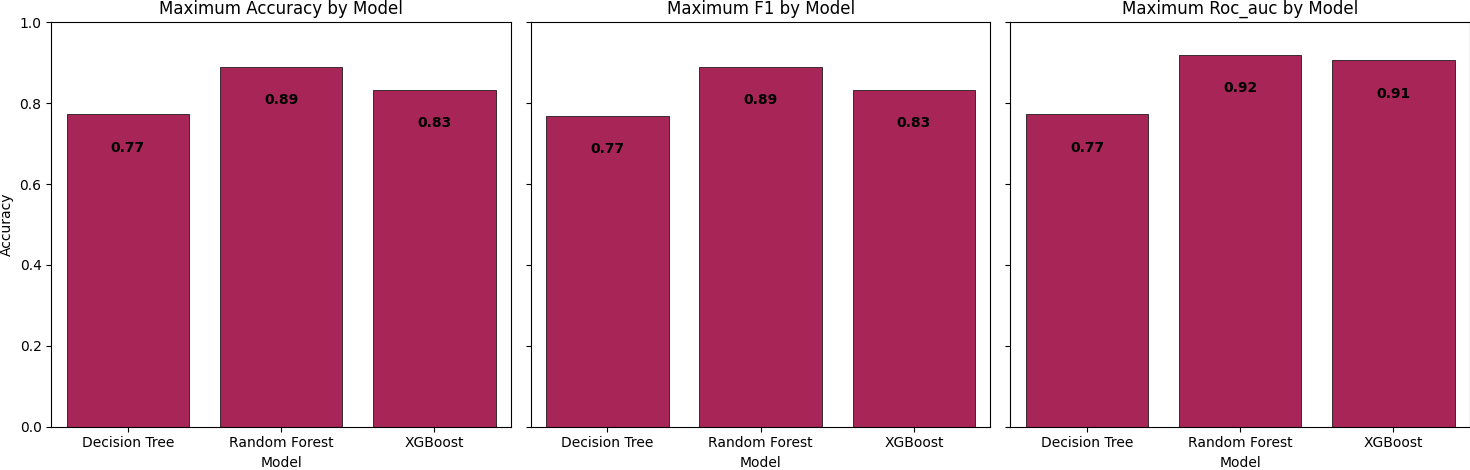
\includegraphics[width=460px]{ModelOptimization/barplots_max_metric.png}%
\caption{Barplots of maximum values of metrics achievied by model}%
\end{figure}

%
\newpage%
\section{Interpretabilty of the best models}%
\label{sec:Interpretabiltyofthebestmodels}%
Auto2class package defined the best model as the one that achievied the highest value of a metric, chosen by the user, or ROC AUC by default.%
In this case, the optimization process was aimed at maximizing%
\textbf{ Accuracy.}%
\\%
Do not forget, that after preprocessing, columns names have changed, because of transformations of categorical features.%
\subsection{The best XGBoost model Explanation}%
\label{subsec:ThebestXGBoostmodelExplanation}%


\begin{figure}[h!]%
\centering%
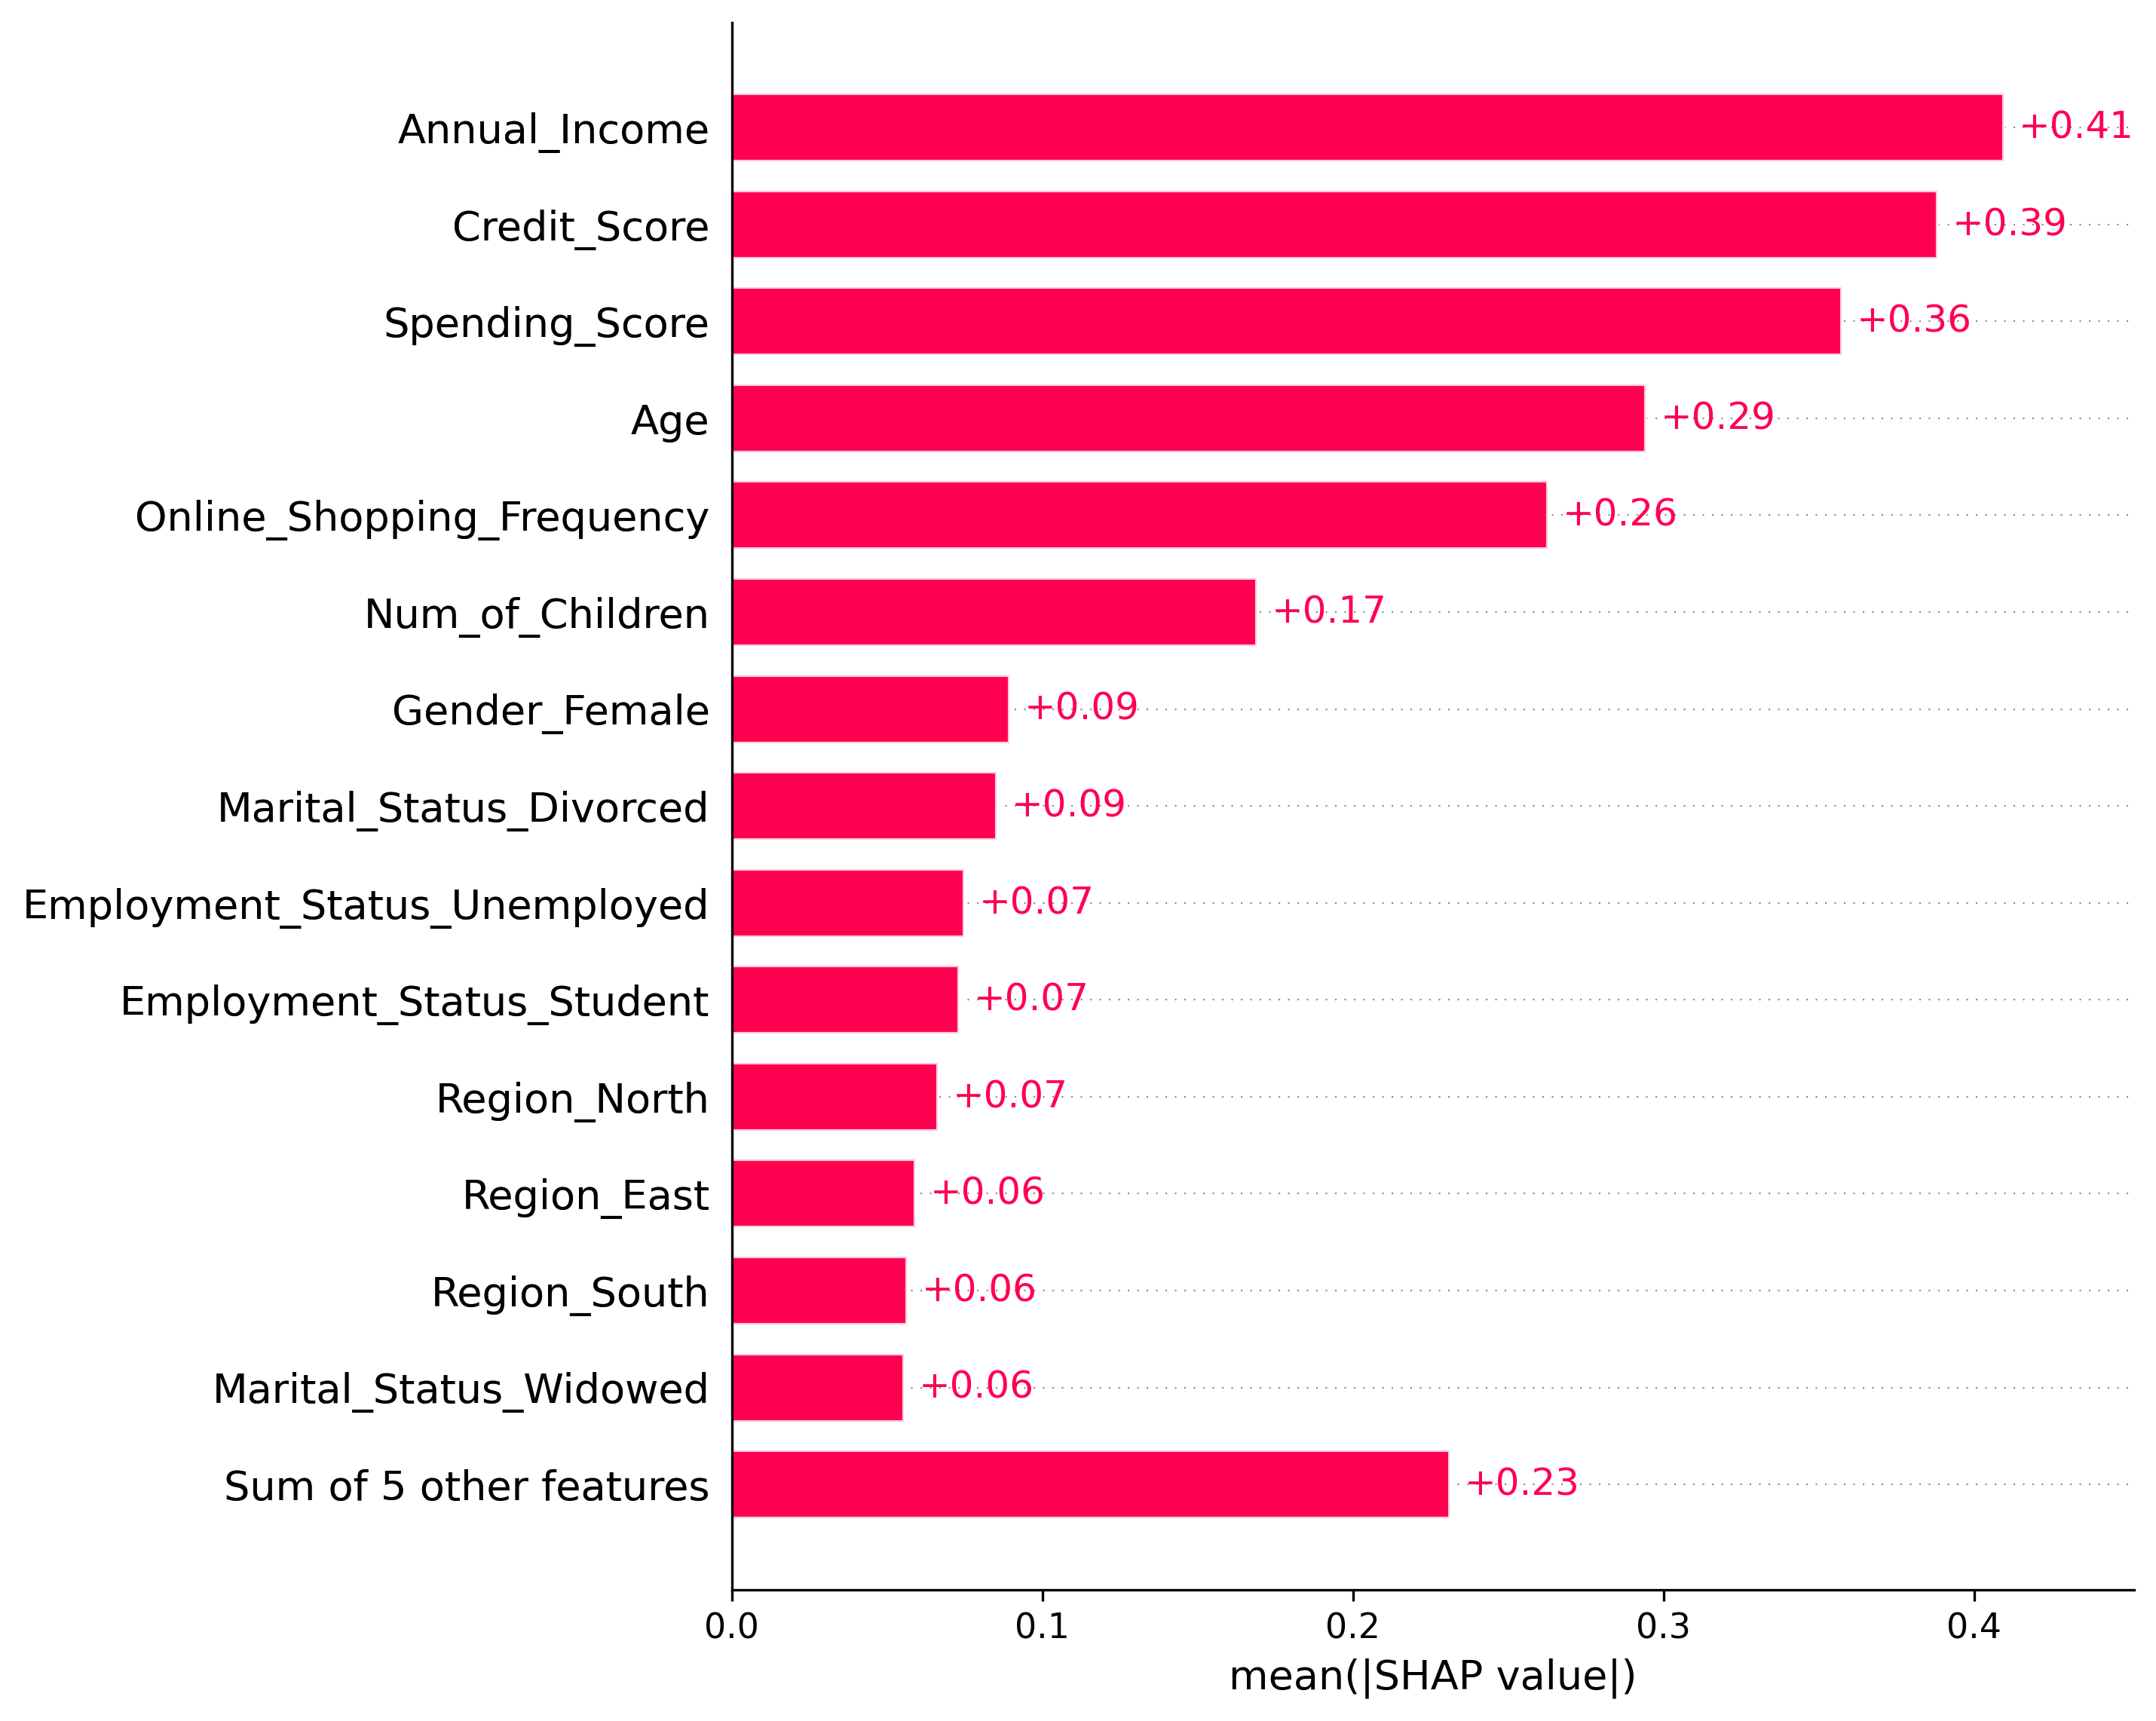
\includegraphics[width=350px]{XAI/XGBoost/global_feature_importance_shap.png}%
\caption{SHAP values for the best XGBoost model}%
\end{figure}

%


\begin{figure}[h!]%
\centering%
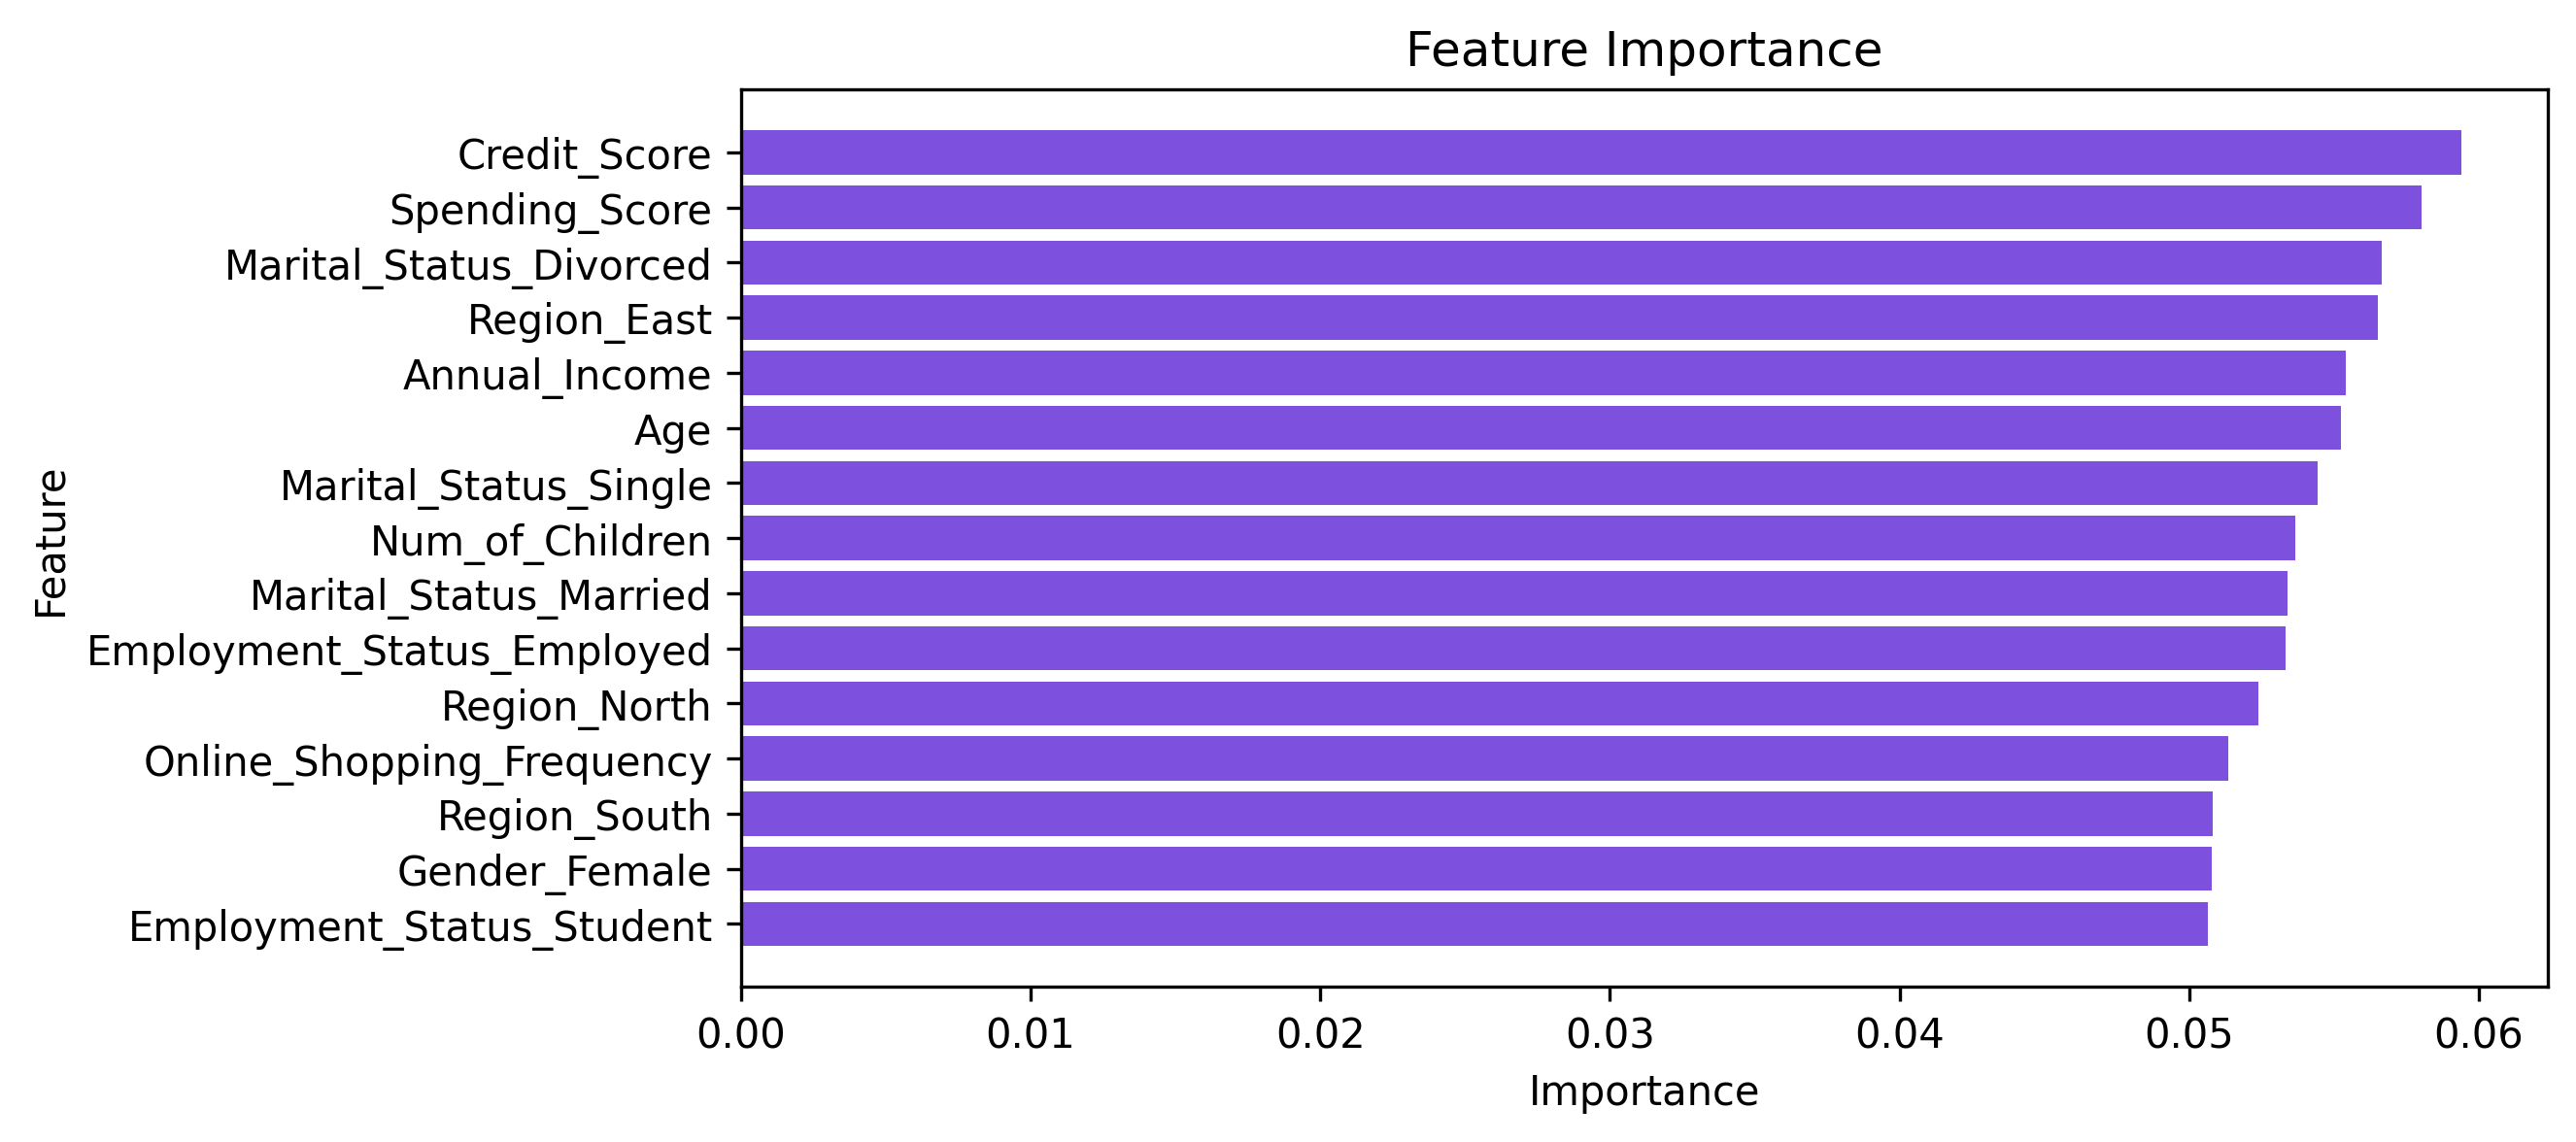
\includegraphics[width=350px]{XAI/XGBoost/feature_importance.png}%
\caption{Feature Importance for the best XGBoost model}%
\end{figure}

%


\begin{figure}[h!]%
\centering%
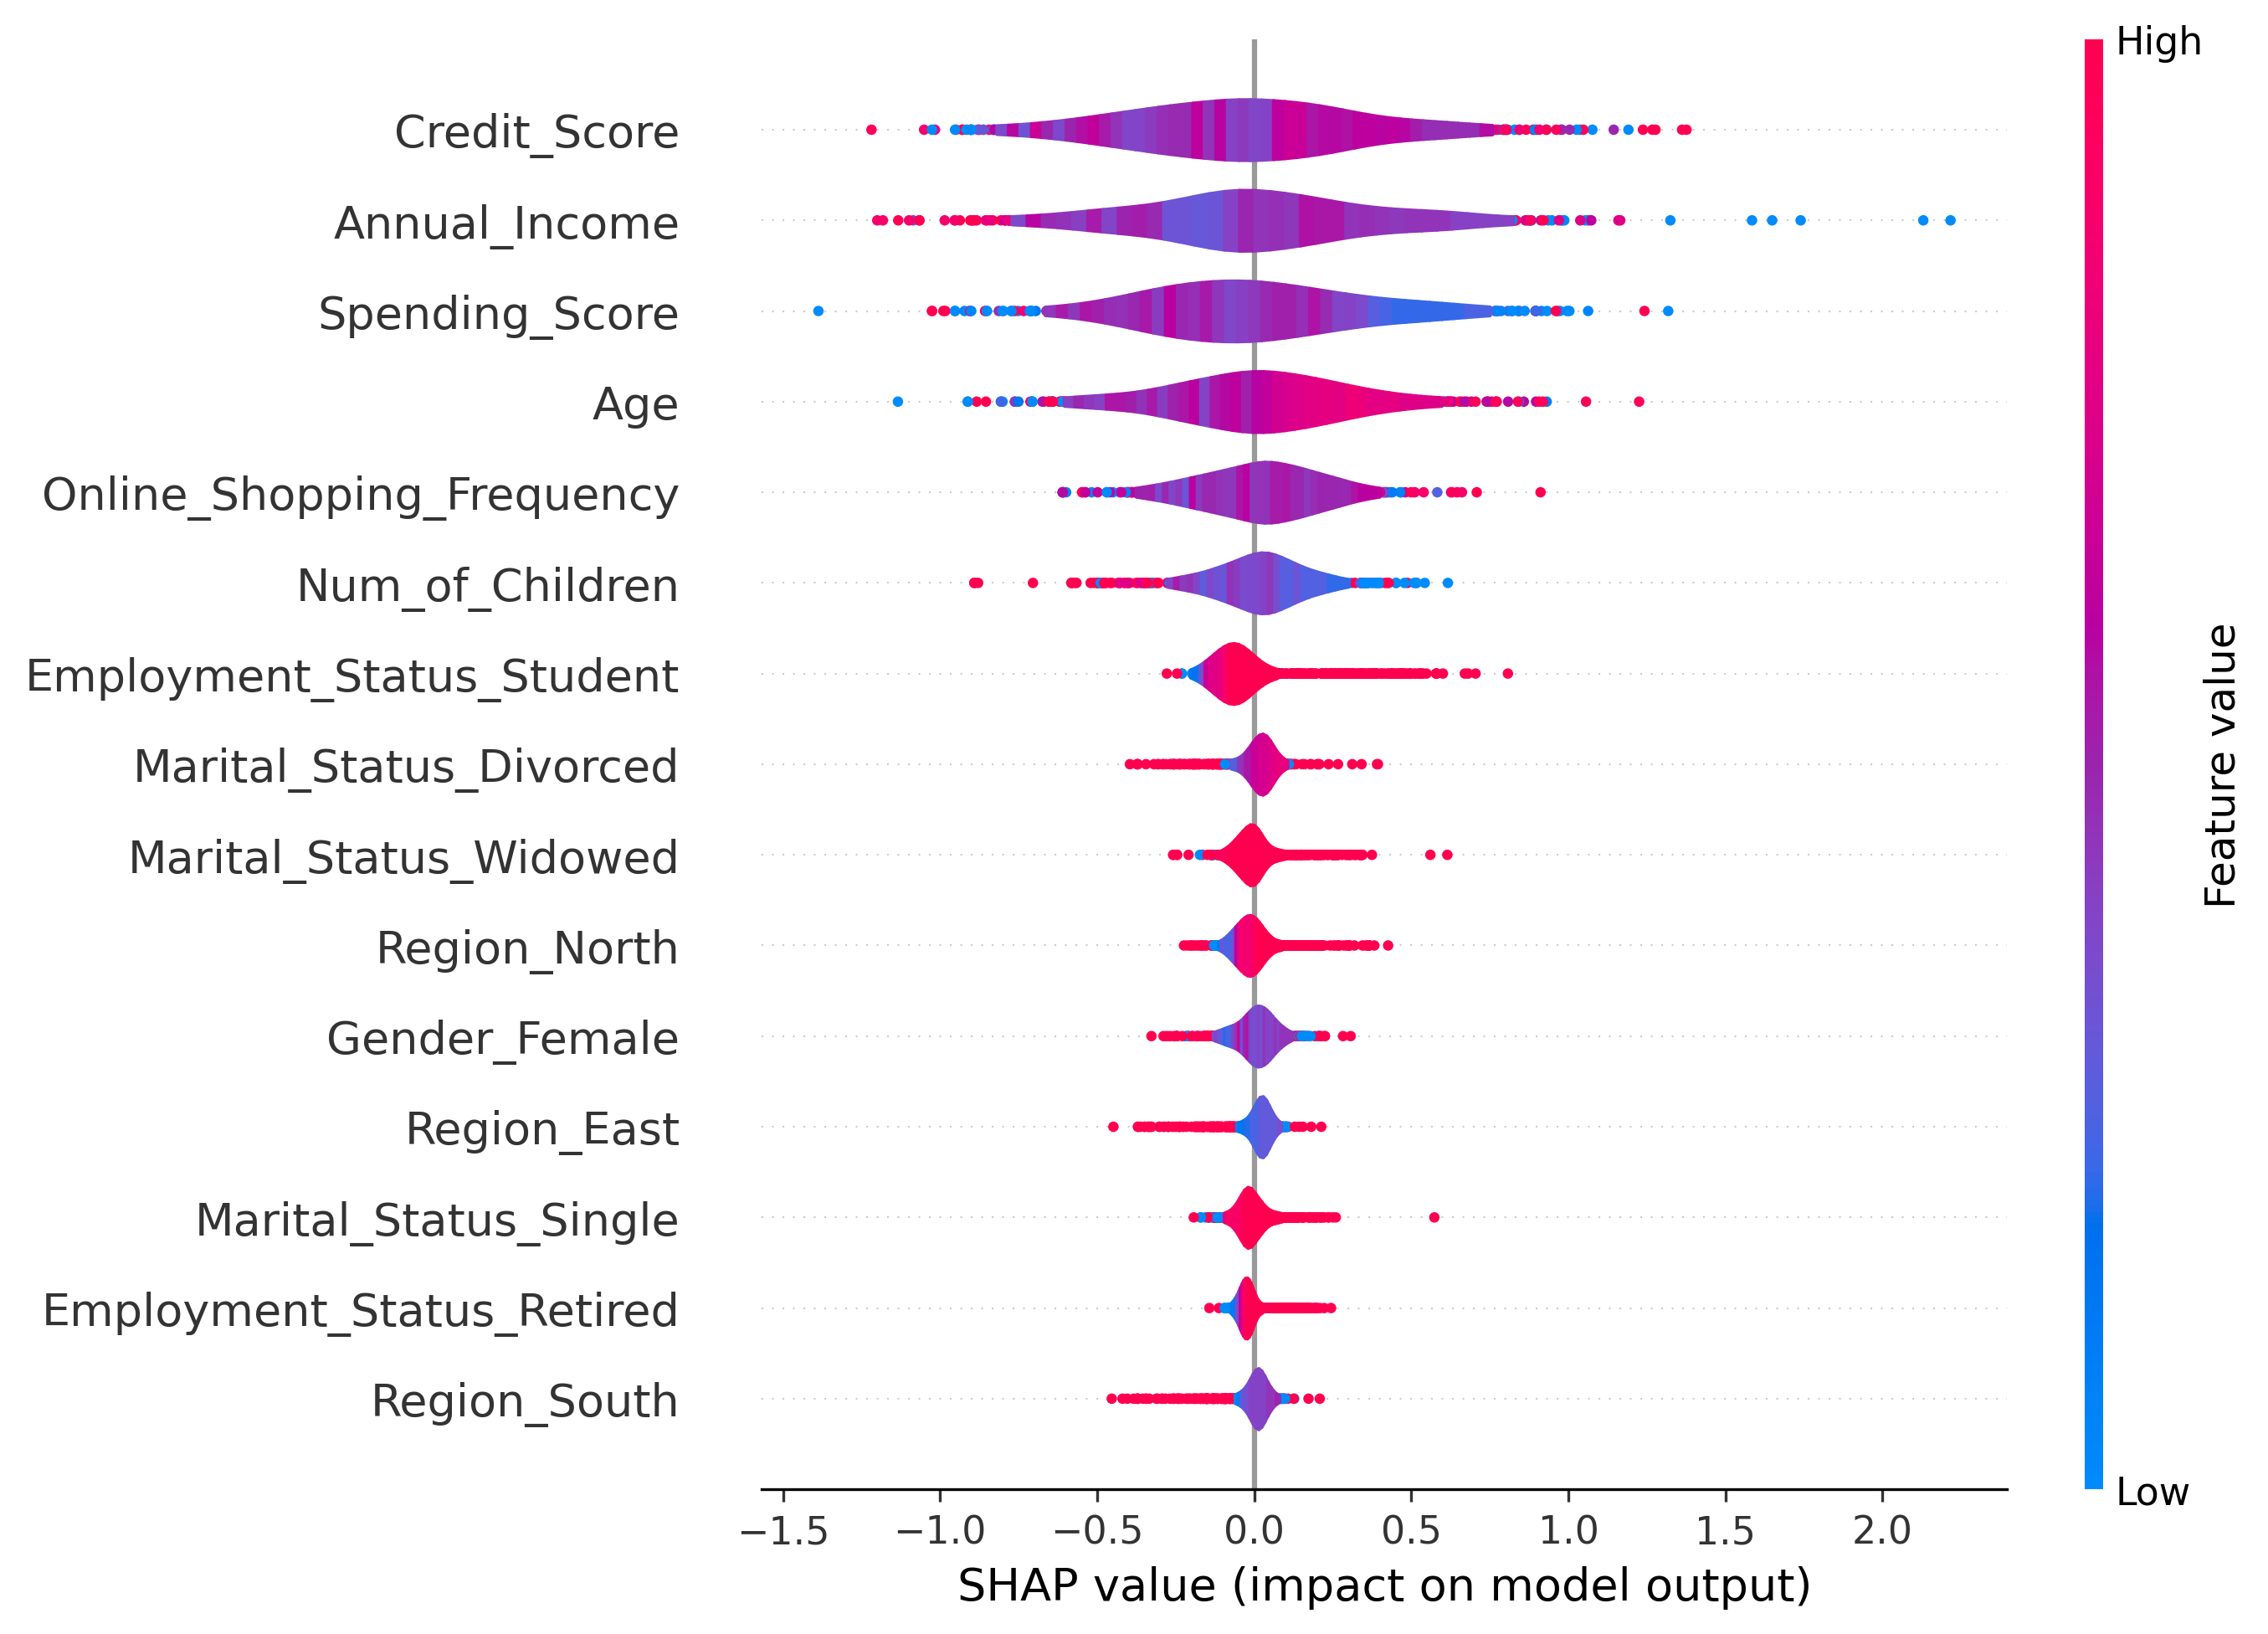
\includegraphics[width=400px]{XAI/XGBoost/violin_summary_plot_shap.png}%
\caption{Violin plot (SHAP) of impact on prediction for the best default XGBoost model}%
\end{figure}

%
\end{document}